\subsection{Gegenseitige Validierung der Suchalgorithmen}

Die beiden Suchalgorithmen können verwendet werden, um deren Ergebnisse gegenseitig zu validieren. Ein ähnliches Verfahren wird beispielsweise in \cite{intradbvalid} verwendet, um bekannte Diagnosen in der gleichen Datenbank über die Auswertung anderen Daten zu bestätigen.

Das Ergebnis der horizontalen Suche für ICD-10-GM Kode G83.8, ausgehend von Version 1.3 ist in Abbildung \ref{hori-umst} dargestellt. Analog kann das Ergebnis der vertikalen Suche über die ConceptMap für ICD-10-GM mit Zielversion 2024 bestimmt werden. Zum Beispiel unter Verwendung von cURL \cite{curl} und HAPI:

\begin{Code}
curl -X 'POST' \
  'http://localhost:8080/fhir/ConceptMap' \
  -H 'accept: application/fhir+json' \
  -H 'Content-Type: application/fhir+xml' \
  -d "@/home/simon/Downloads/conceptmap_r4_icd10gm_2024.xml"
\end{Code}

\begin{Code}
curl -X 'GET' \
  'http://localhost:8080/fhir/ConceptMap/$translate?code=G83.8&system=1.3' \
  -H 'accept: application/fhir+json'
\end{Code}

\begin{comment}
\newpage

\begin{Code}
{
  "resourceType": "Parameters",
  "parameter": [ {
    "name": "result",
    "valueBoolean": true
  }, {
    "name": "message",
    "valueString": "Matches found"
  }, {
    "name": "match",
    "part": [ {
      "name": "equivalence",
      "valueCode": "wider"
    }, {
      "name": "concept",
      "valueCoding": {
        "system": "2024",
        "code": "G83.6"
      }
    }, {
      "name": "source",
      "valueUri": "urn:uuid:0192f4d0-20da-7a03-9f2e-a50d9266aeee"
    } ]
  }, {
    "name": "match",
    "part": [ {
      "name": "equivalence",
      "valueCode": "wider"
    }, {
      "name": "concept",
      "valueCoding": {
        "system": "2024",
        "code": "G83.8"
      }
    }, {
      "name": "source",
      "valueUri": "urn:uuid:0192f4d0-20da-7a03-9f2e-a50d9266aeee"
    } ]
  }, {
    "name": "match",
    "part": [ {
      "name": "equivalence",
      "valueCode": "wider"
    }, {
      "name": "concept",
      "valueCoding": {
        "system": "2024",
        "code": "G83.5"
      }
    }, {
      "name": "source",
      "valueUri": "urn:uuid:0192f4d0-20da-7a03-9f2e-a50d9266aeee"
    } ]
  } ]
\end{Code}
\end{comment}


\begin{comment}
\begin{Code}
curl -X 'POST' \
  'http://localhost:8080/fhir/ConceptMap' \
  -H 'accept: application/fhir+json' \
  -H 'Content-Type: application/fhir+xml' \
  -d "@/home/simon/Downloads/conceptmap_r4_icd10gm_2024.xml"
\end{Code}

\begin{Code}
curl -X 'GET' \
  'http://localhost:8080/fhir/ConceptMap/$translate?code=G83.8&system=1.3' \
  -H 'accept: application/fhir+json'
\end{Code}
\end{comment}

Das Ergebnis ist ebenfalls: [G83.6, G83.8, G83.5]. Natürlich kann der Vergleich der beiden Suchalgorithmen auch programmiert werden. 

\subsection{Qualität der Mappings}

Die durch diese Arbeit generierten ConceptMaps können anhand der Qualitätsstandards aus Abschnitt \ref{quali-map} beurteilt werden:

\begin{enumerate}
\item Einsatzzweck und Umfang der ConceptMaps sind klar definiert sein. Mappings erfolgen zwar chronologisch in zwei Richtungen, aber mit dem gleichen Algorithmus.
\item Die ConceptMaps richten sich nach den vom BfArM erstellten Überleitungstabellen.
\item Als Masterarbeit sind die Anforderung an das Team nicht erfüllt. Vertreter des BfArMs waren nicht beteiligt. 
\item Diese Arbeit dokumentiert das Mapping und der Programmcode ist frei verfügbar. 
\item Getestet wurde automatisiert durch Abgleich der zwei Suchalgorithmen, aber manuell nur stichprobenartig.
\item Der Datenintegrationsprozess wurde bewusst so entworfen, dass ein Update auf neue Versionen möglichst einfach ist. Änderungen am Programmcode sind nur notwendig, wenn sich die BfArM-Daten oder deren Veröffentlichung essentiell ändern. 
\item FHIR ConceptMaps erfordern die Definition von Kardinalität, Relationen, sowie Ursprung- und Zielversion des Mappings.
\item FHIR ConceptMaps sind maschinell lesbar.
\end{enumerate}

\section{Zusammenfassung}

Es wurden zwei Suchalgorithmen zur Bestimmung von Umsteigern über alle Versionen der ICD-10-GM und des OPS vorgestellt. Einer dient zum Abbilden vieler Informationen zu einzelnen Kodes und der andere zur effizienten Erstellung von ConceptMaps. Beide Varianten können interoperabel eingesetzt werden. Die Aufnahme von neuen Versionen sollte durch den Datenintegrationsprozess gewährleistet sein. Wichtig ist noch das manuelle Testen der Mappings. 

\newpage

\section{Ausblick}

Folgende Weiterentwicklungen sind sinnvoll.

\subsection{RESTful}

Die Web-Applikation sollte nicht nur teilweise, sondern komplett dem REST-Paradigma entsprechen, wie in Abschnitt \ref{rest-paradigm} aufgeführt. Das bedeutet alle Informationen des Servers durch Schnittstellen bereitzustellen: 

\begin{itemize}
\item Kodes pro System und Version als FHIR "`Code System"' Ressourcen zum Download.
\item Umsteiger pro Version im JSON-Format per API-Schnittstelle. Die Übersichtsseite für Umsteiger lädt aktuell schon relativ lange aufgrund der Menge an Daten und das könnte per AJAX beschleunigt werden, das bedeutet Laden der Umsteiger jeweils nur für die angezeigte Version. 
\item Ergebnis der horizontalen Suche im JSON-Format per API-Schnittstelle. Ähnlich wie der Modal-Content, aber ohne Formatierung für die Anzeige.
\item ConceptMaps per API-Schnittstelle ohne Formular, welches nur manuell ausgefüllt werden kann. 
\end{itemize}

Außerdem sollten die Schnittstellen dokumentiert sein über Swagger UI \cite{swagger}.

Bei einem wirklich produktiv eingesetzten System wäre es sinnvoll Daten zu cachen:

\begin{itemize}
\item Umsteiger-Ergebnisse der horizontalen Suche. 
\item ConceptMap-Dateien, damit diese nicht immer neu generiert werden müssen. 
\end{itemize}

Das würde allerdings sehr viel mehr an Speicherplatz belegen. 

\subsection{ATC}

Das BfArM stellt neben ICD-10-GM und OPS auch die deutsche Version der ATC Klassifikation, \emph{Anatomical Therapeutic Chemical}, zur Verfügungen unter \cite{bfarmatc}. Diese wird im Auftrag durch die WIdO erstellt, dem Wissenschaftliche Institut der Allgemeinen Ortskrankenkassen. Die Klassifikations- und Änderungsdateien gibt es nur als PDF. Die Aufnahme von ATC in den \bfarmer-Datenintegrationsprozess würde also einen PDF-Parser erfordern. 

Mit \cite{poppler} können PDF-Dateien in XML-Dateien umgewandelt werden:

\begin{Code}
pdftohtml atc-vergleichsdatei-amtlich-2024-2023.pdf test.xml -nodrm -i -xml
\end{Code}

Das Parsen wird dadurch vereinfacht, dass alle Tabellen in den ATC PDF-Dateien mit "`Tabelle"' + Zahl beginnen und mit "`Quelle: GKV-Arzneimittelindex im Wissenschaftlichen Institut der AOK (WIdO)"' enden. Zum Beispiel: 

\begin{figure}[H]
    \centering
    \setlength{\fboxsep}{12pt}\color{black!20}\fbox{
    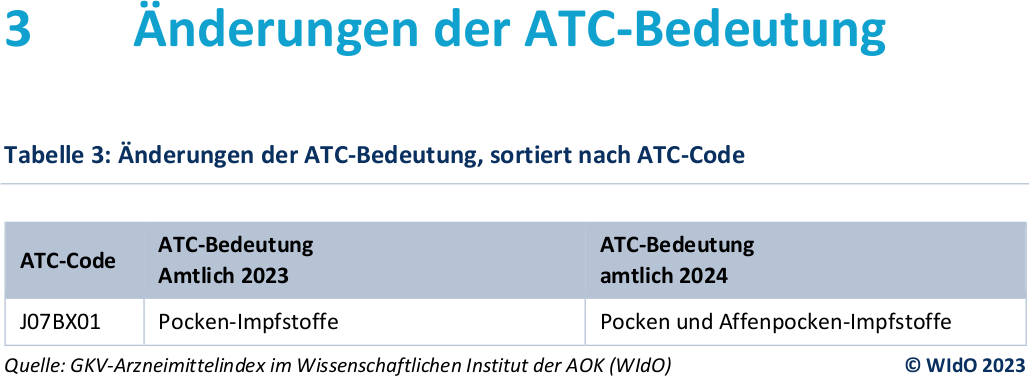
\includegraphics[width=.99\linewidth]{../img/atc.png}}
    \normalcolor\caption{Beispiel Überleitungstabelle in einer ATC PDF-Datei.}
\end{figure}

\vspace{-1em}

Die konvertierte XML-Datei enthält Text immer in \texttt{<text>}-Tags und durch Auslesen des Inneren dieser Tags ergibt sich: 

\begin{Code}
<b>Tabelle 3: Änderungen der ATC-Bedeutung, sortiert nach ATC-Code </b>
<b>ATC-Code </b>
<b>ATC-Bedeutung  </b>
<b>Amtlich 2023 </b>
<b>ATC-Bedeutung  </b>
<b>amtlich 2024 </b>
J07BX01
Pocken-Impfstoffe
Pocken und Affenpocken-Impfstoffe
<i>Quelle: GKV-Arzneimittelindex im Wissenschaftlichen Institut der AOK (WIdO) </i>
<b>© WIdO 2023 </b>
\end{Code}

Die Tabellen können eine unterschiedliche Anzahl an Spalten haben, aber die Anzahl sowie die Überschrift bleibt pro Tabellentyp gleich. Die Zeilen beginnen immer mit einem Kode und dieser könnte per regulärem Ausdruck identifiziert werden. Es müssten anhand der unterschiedlichen Tabellen Umsteiger-Informationen analog zu ICD-10-GM und OPS generiert werden. Außerdem müsste die Information über DDD, die definierte Tagesdosis, als zusätzliche Tabelle gespeichert und extra für ATC angezeigt werden. 

\subsection{Sessions}

Ein Session-Management würde es ermöglichen, dass nicht nur die Zielversion, sondern auch die Ausgangsversionen für ConceptMaps wählbar sind. Aktuell sind immer alle Versionen ausgewählt, aber das könnte zum Beispiel durch Checkboxen einstellbar gemacht werden. Diese Einstellungen müssen allerdings als Session-Informationen gespeichert werden. Das ist Client- und Server-seitig möglich. Client-seitig würde den Einbau eines Cookie-Banners notwendig machen. Server-seitig ist es komplizierter umzusetzen und erfordert zusätzlichen Speicherplatz in der Datenbank. 

